\section{What is an \ab{} workflow system?}

\subsection{What are \ab{} calculations?}

\begin{frame}{What are \ab{} calculations?}
    \begin{definitionblock}{\ab{} calculation}
        A method of calculating atomic and molecular structure directly from the first
        principles of quantum mechanics, without using quantities derived from experiment
        as parameters.
    \end{definitionblock}

    \begin{itemize}
        \item Electronic structure computation
        \item Optimize input crystal/molecular structures
        \item Phonon vibrational spectra computation
        \item Helmholtz free energy calculation at finite temperature
        \item Linear elastic constants
        \item More...
    \end{itemize}
\end{frame}

\begin{frame}{Typical \ab{} workflows used in our group}
    \begin{figure}[H]
        \centering
        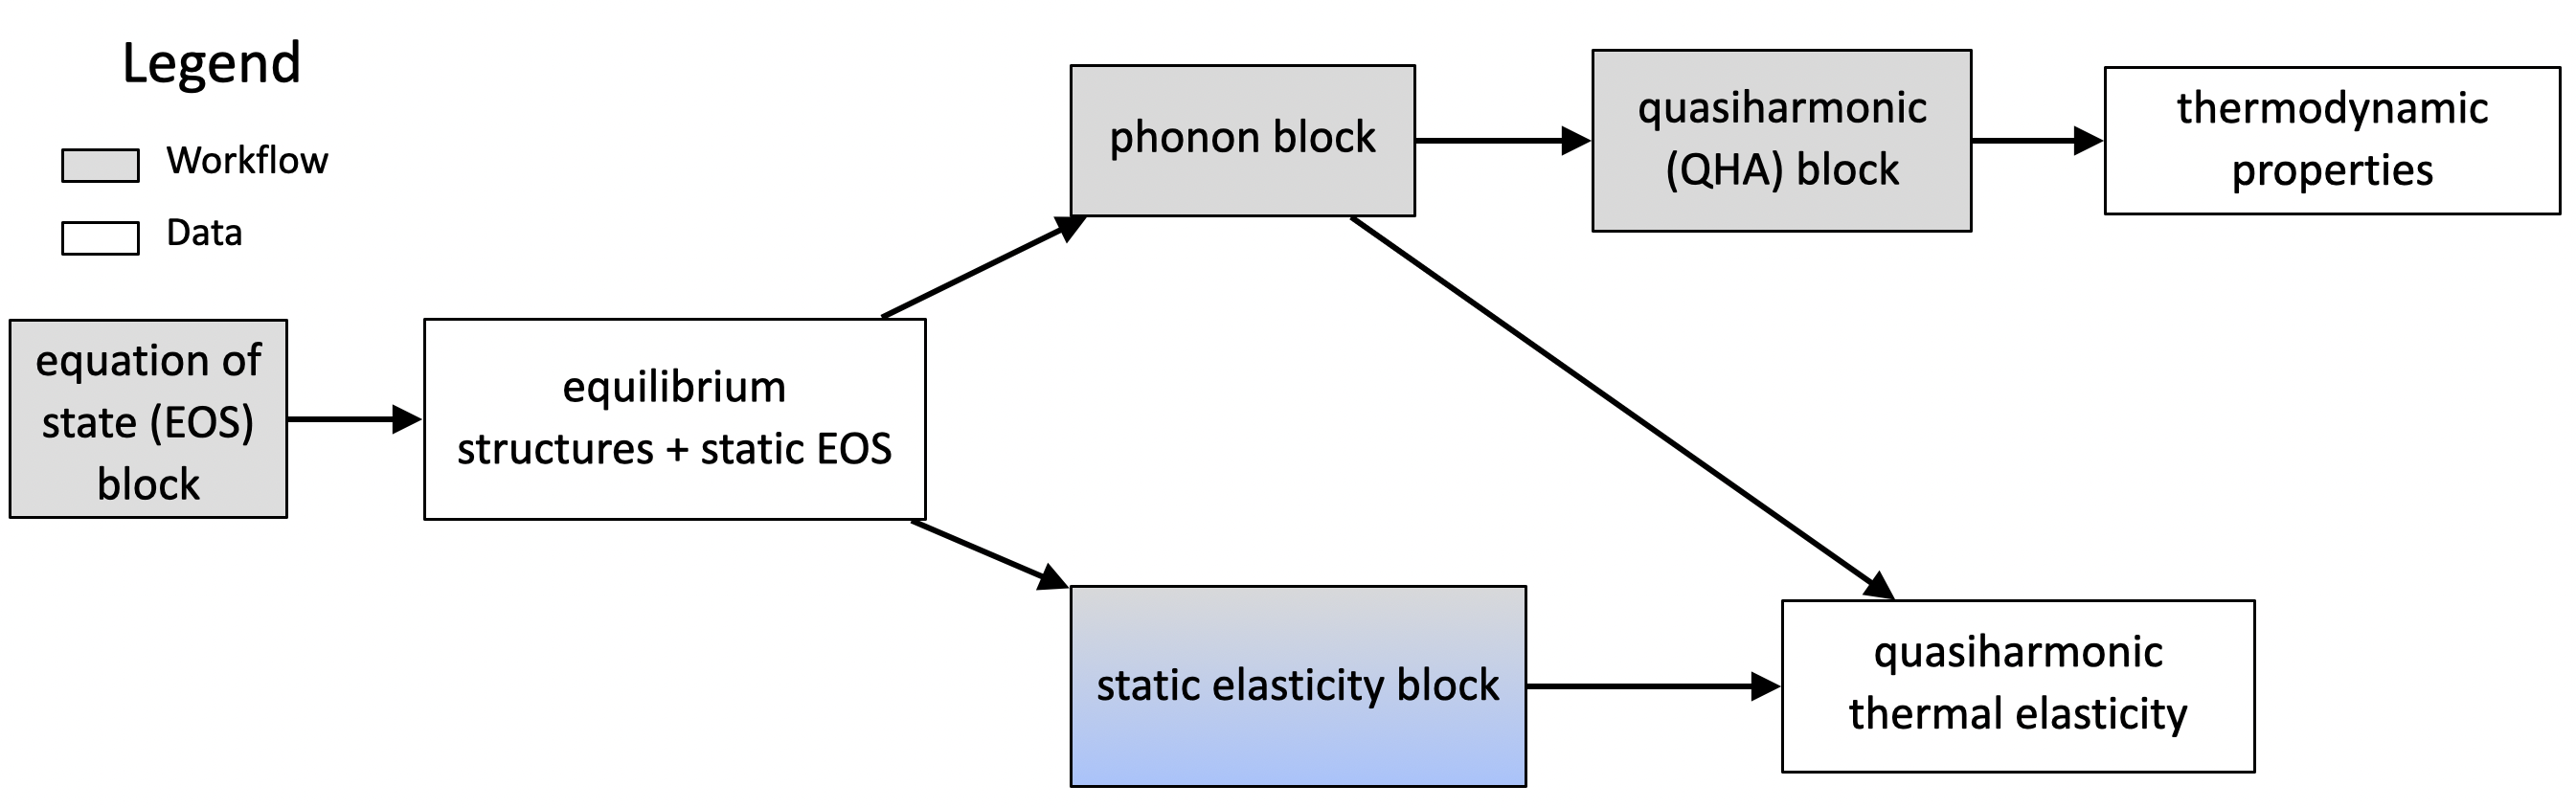
\includegraphics[height=0.4\textheight]{workflows}
        \label{eq:workflows}
    \end{figure}
\end{frame}

\begin{frame}{Various \ab{} software}
    To do \ab{} calculations, it is inevitable to interact with \ab{} software.
    There are a lot of them on the market, e.g., \qe{}, VASP, and ABINIT.
    They are often written in Fortran, and needed to be compiled to executable
    when using.

    So building a workflow for them requires us to create parsers for their input and output
    files, as well as functions to dynamically run these executables.

    \begin{figure}[b]
        \centering
        
\includegraphics[width=0.4\textwidth]{qe}
        \hfill
        
\includegraphics[width=0.2\textwidth]{vasp}
        \hfill
        
\includegraphics[width=0.3\textwidth]{abinit}
        \label{fig:abinitsoftware}
    \end{figure}
\end{frame}
\subsection{What is needed in an \ab{} workflow system?}

\begin{frame}{What is needed in an \ab{} workflow system?}
    There are at least three components:

    \begin{itemize}
        \item Sciency, technical stuff: calculations, input generation, output analysis...
        \item Dispatcher, job scheduler: interacting with \ab{} software, \texttt{mpi}...
        \item User interface: interacting with users
    \end{itemize}
\end{frame}

\subsection{What is \express{}?}

\begin{frame}{What is \express{}?}
    \begin{definitionblock}{\express{}}
        A workflow framework consisting of several extensible, lightweight, high-throughput,
        high-level Julia packages that aims to automate \ab{} calculations for the materials
        science community.
    \end{definitionblock}

    \begin{definitionblock}{\texttt{Express.jl}}
        The core package of the \express{} project, which manages and dispatches the rest
        packages in \express{}.
    \end{definitionblock}
\end{frame}

\begin{frame}[allowframebreaks]{What does the \express{} project include?}
    \begin{figure}
        \centering
        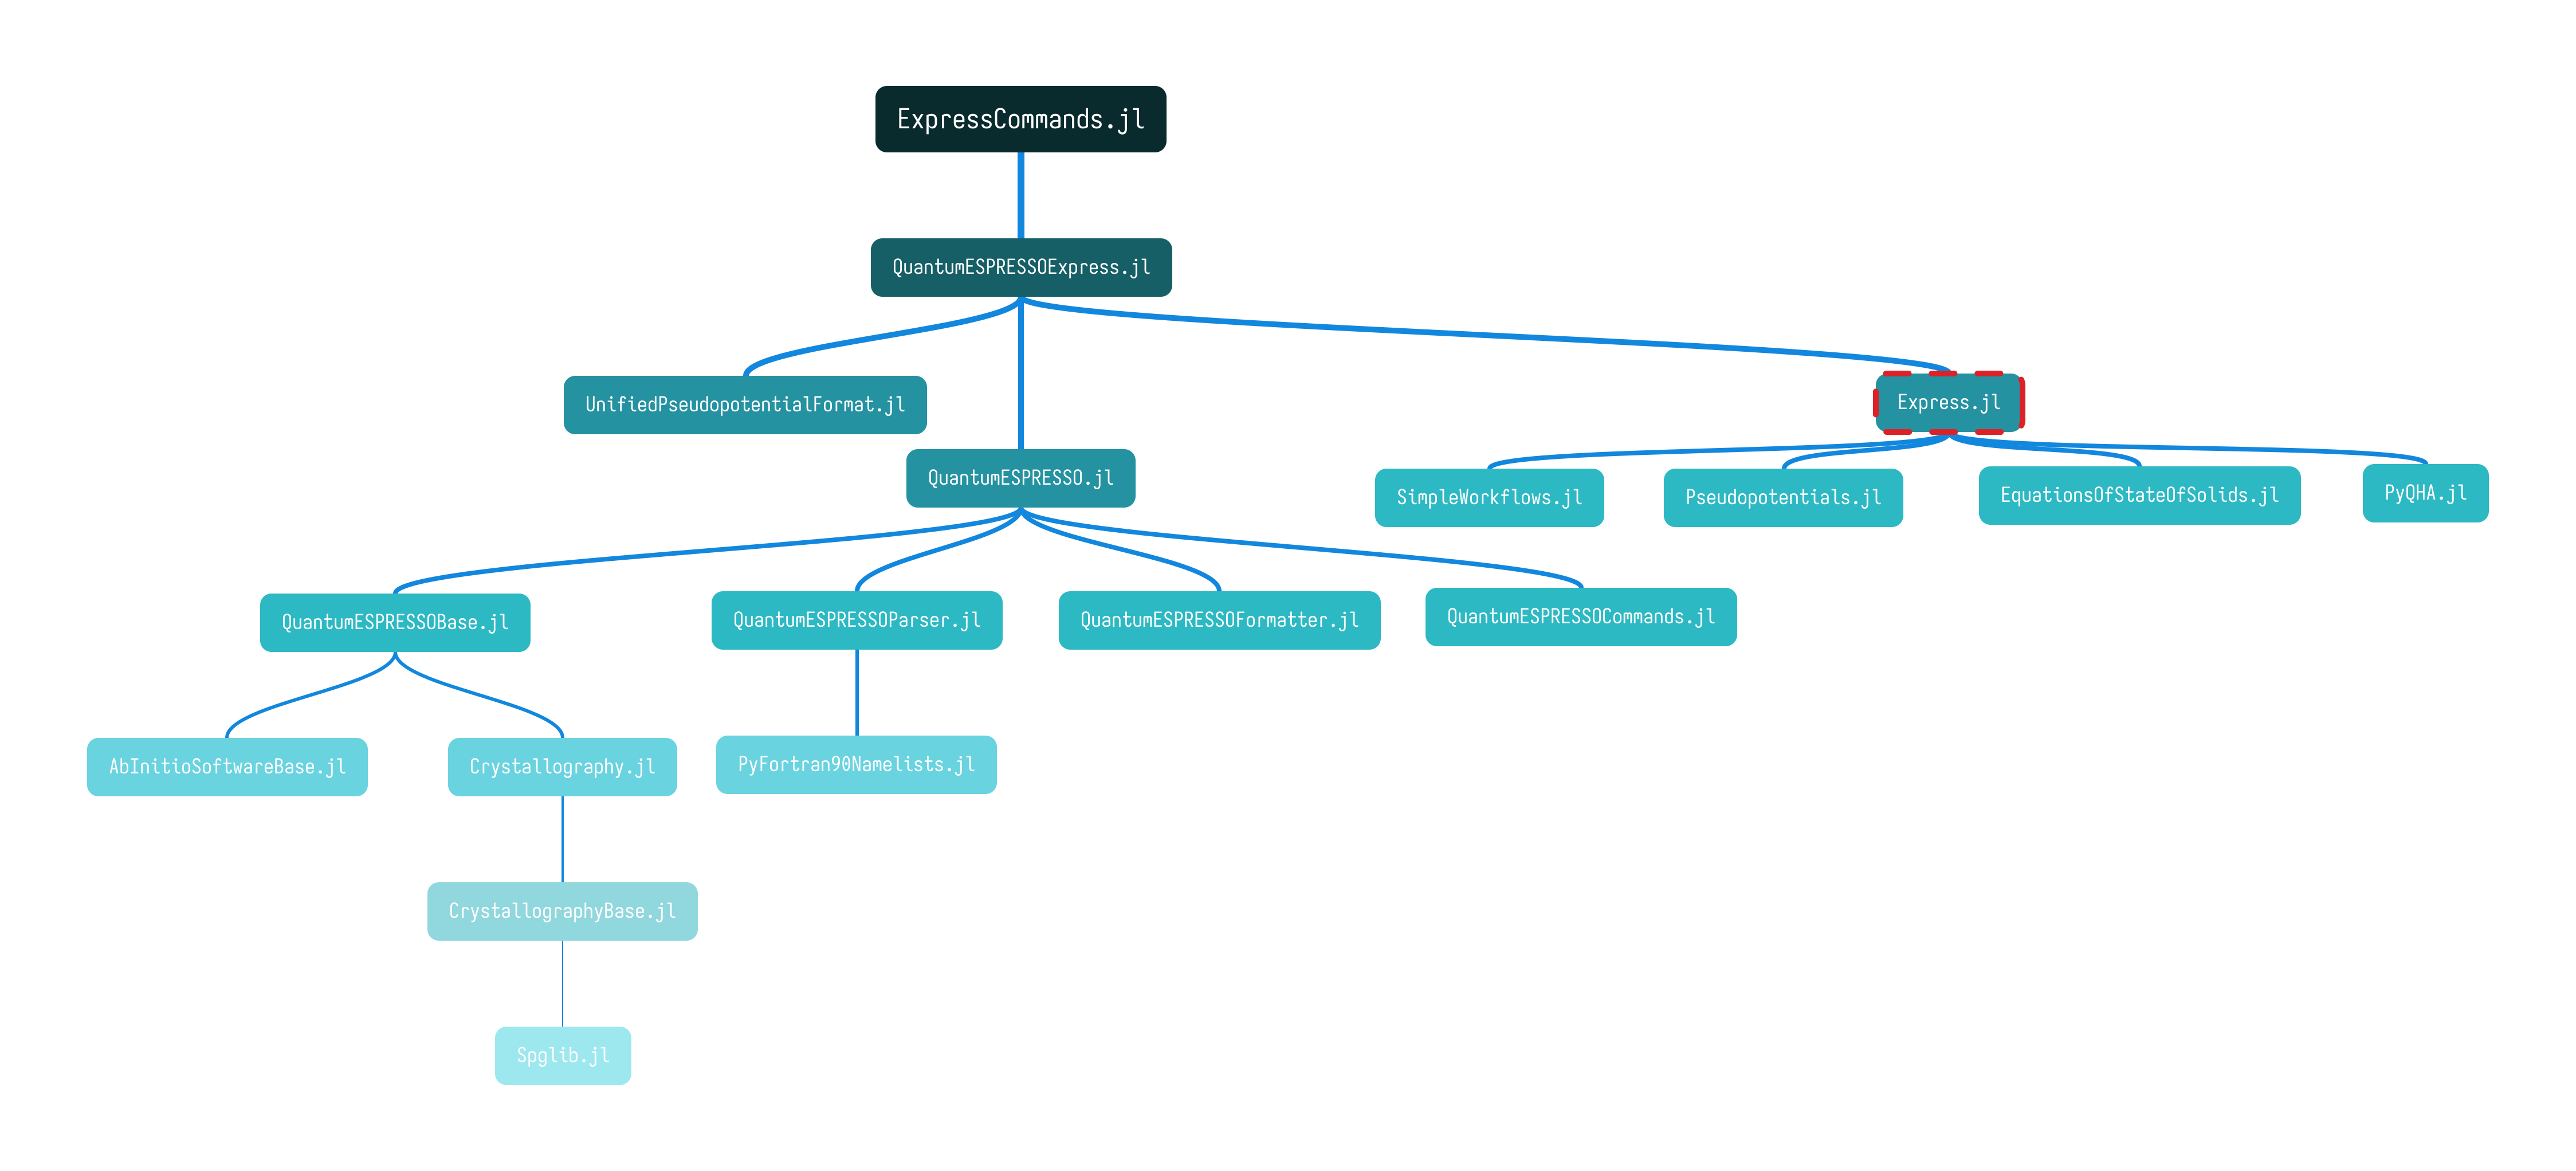
\includegraphics[width=\textwidth]{components}
        \label{fig:components}
    \end{figure}

    \begin{itemize}
        \item \href{https://github.com/MineralsCloud/Express.jl}{\texttt{Express.jl}}
              provides a high-level interface to all the
              workflows, including file reading and writing, job
              creation, submission, monitoring, result retrieving, and data
              analysis. To work with specific software, install the corresponding plugin,
              e.g., \texttt{QuantumESPRESSOExpress.jl} for \qe.
        \item \href{https://github.com/MineralsCloud/ExpressCommands.jl}{\texttt{ExpressCommands.jl}}
              is a user-friendly command-line interface of
              \texttt{Express.jl} for non-developers. It installs an executable
              `\texttt{xps}' that can execute code from configuration files provided by users.
        \item \href{https://github.com/MineralsCloud/EquationsOfStateOfSolids.jl}{\texttt{EquationsOfStateOfSolids.jl}}
              fits energy (or pressure) vs. volume results to equations of state,
              etc. These features are repetitively used in the equation of state workflow.
        \item \href{https://github.com/MineralsCloud/Crystallography.jl}{\texttt{Crystallography.jl}}
              calculates a crystal's primitive cell (or supercell) volume from lattice parameters, finds symmetry
              operations and generates high symmetry points in the Brillouin zone, etc.
        \item \href{https://github.com/MineralsCloud/PyQHA.jl}{\texttt{PyQHA.jl}}
              is a Julia wrapper of
              the Python \texttt{qha} package, which can calculate
              several thermodynamic properties of both single- and multi-configuration
              crystalline materials in the framework of quasi-harmonic approximation.
        \item \href{https://github.com/MineralsCloud/Pseudopotentials.jl}{\texttt{Pseudopotentials.jl}} presents
              a database for storing and querying pseudopotentials used in \ab{} calculations.
        \item \href{https://github.com/MineralsCloud/SimpleWorkflows.jl}{\texttt{SimpleWorkflows.jl}}
              is the skeleton of the workflow system, which
              defines building blocks, composition rules, and operation order of workflows.
        \item \href{https://github.com/MineralsCloud/AbInitioSoftwareBase.jl}{\texttt{AbInitio\-Software\-Base.jl}}
              provides a standard API for some popular \ab{} software such as \qe.
        \item \href{https://github.com/MineralsCloud/QuantumESPRESSOBase.jl}{\texttt{Quantum\-ESPRESSO\-Base.jl}}
              declares basic data types and methods
              for manipulating crystal structures, generating input files for \qe,
              error checking before running, etc.
        \item \href{https://github.com/MineralsCloud/QuantumESPRESSOParser.jl}{\texttt{Quantum\-ESPRESSO\-Parser.jl}}
              parses the input or output files of \qe{} to extract and analyze data.
        \item \href{https://github.com/MineralsCloud/QuantumESPRESSOFormatter.jl}{\texttt{Quantum\-ESPRESSO\-Formatter.jl}}
              formats the input files of \qe.
        \item \href{https://github.com/MineralsCloud/QuantumESPRESSOCommands.jl}{\texttt{Quantum\-ESPRESSO\-Commands.jl}}
              is a command-line interface that exports the commands \qe{} uses in a configurable way.
        \item \href{https://github.com/MineralsCloud/QuantumESPRESSO.jl}{\texttt{QuantumESPRESSO.jl}}
              is simply a wrapper of the types, methods, and commands defined in
              \texttt{Quantum\-ESPRESSO\-Base.jl}, \texttt{Quantum\-ESPRESSO\-Parser.jl},
              \texttt{Quantum\-ESPRESSO\-Formatter.jl},
              and \texttt{Quantum\-ESPRESSO\-Commands.jl} under a common namespace.
    \end{itemize}
\end{frame}
